\section{Test day}

\subsection{What the test looks like}
Test 1 is in your discussion section on Thursday Oct 15 or Friday Oct 16, depending on which section you're in. The review session is the day before, so don't mix those up. It's closed book, closed notes, no devices, with one exception: a single 8.5$\times$11 sheet with whatever you want written on it. The rules don't say whether both sides count or whether printed is fine, so ask your TA rather than guessing.

Expect three kinds of question:
\begin{itemize}
\item \textbf{Compute something.} Work out a set, a truth table, a power set, a degree or an output set. These are quick points if you're careful.
\item \textbf{Decide and justify.} Is the claim true or false? Then back it up with the evidence that kind of claim needs (the obligation table in Chapter 2). A bare ``true'' usually earns nothing.
\item \textbf{Write or check a proof.} Either write a constrained proof, or read one and label each step's rule, marking the step that's invalid. This is where the test is won or lost.
\end{itemize}

\subsection{The note sheet}
The sheet can't write a proof for you, so don't fill it with proofs. Give it lookup jobs: things you'd otherwise have to reconstruct under pressure. Here's a layout that fits on one side.

\begin{figure}[H]\centering
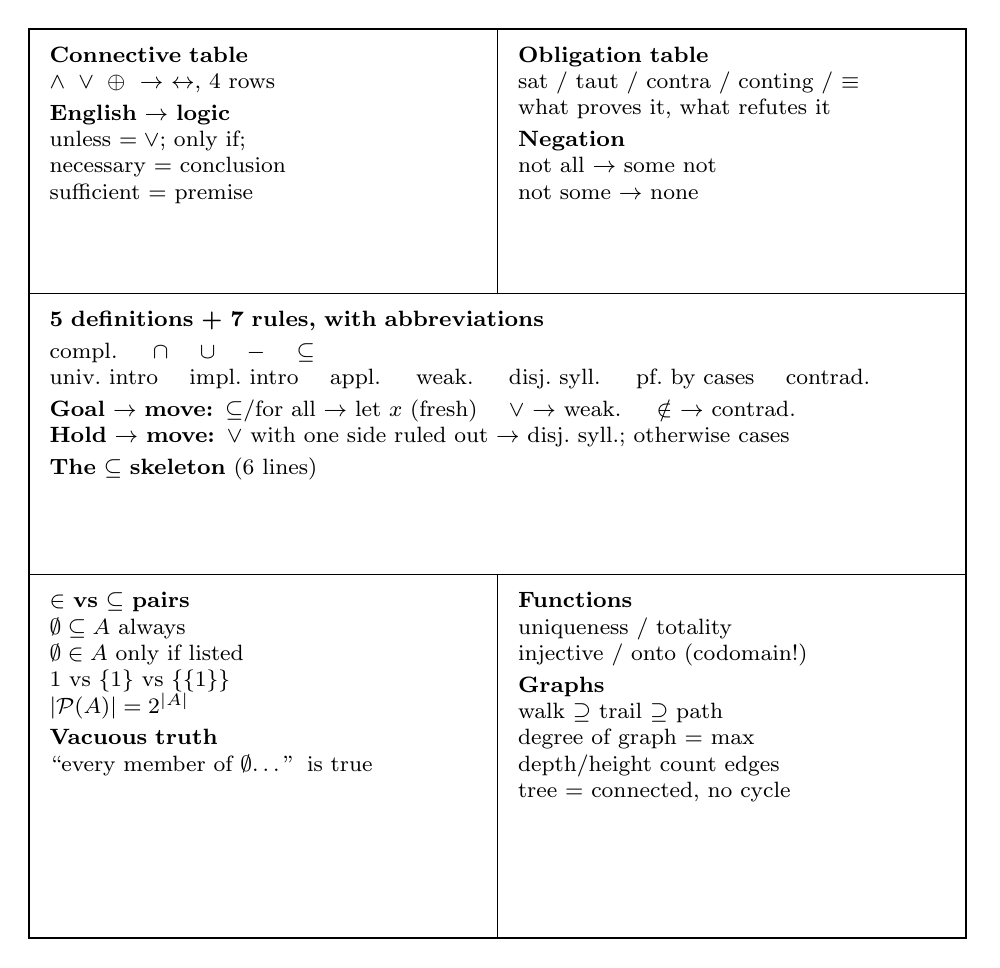
\begin{tikzpicture}[x=1.4cm,y=1.05cm,every node/.style={font=\footnotesize,align=left,anchor=north west}]
  \draw[line width=0.8pt] (0,0) rectangle (8.5,-11);
  \draw (0,-3.2) -- (8.5,-3.2);
  \draw (4.25,0) -- (4.25,-3.2);
  \draw (0,-6.6) -- (8.5,-6.6);
  \draw (4.25,-6.6) -- (4.25,-11);
  \node[text width=5.6cm] at (0.1,-0.1) {\textbf{Connective table}\\ $\land\ \lor\ \oplus\ \to\ \leftrightarrow$, 4 rows\\[2pt] \textbf{English $\to$ logic}\\ unless $=\lor$; only if;\\ necessary = conclusion\\ sufficient = premise};
  \node[text width=5.6cm] at (4.35,-0.1) {\textbf{Obligation table}\\ sat / taut / contra / conting / $\equiv$\\ what proves it, what refutes it\\[2pt] \textbf{Negation}\\ not all $\to$ some not\\ not some $\to$ none};
  \node[text width=11.6cm] at (0.1,-3.3) {\textbf{5 definitions + 7 rules, with abbreviations}\\[2pt]
    compl. \quad $\cap$ \quad $\cup$ \quad $-$ \quad $\subseteq$\\
    univ.\ intro \quad impl.\ intro \quad appl. \quad weak. \quad disj.\ syll. \quad pf.\ by cases \quad contrad.\\[2pt]
    \textbf{Goal $\to$ move:} $\subseteq$/for all $\to$ let $x$ (fresh) \quad $\lor$ $\to$ weak. \quad $\notin$ $\to$ contrad.\\
    \textbf{Hold $\to$ move:} $\lor$ with one side ruled out $\to$ disj.\ syll.; otherwise cases\\[2pt]
    \textbf{The $\subseteq$ skeleton} (6 lines)};
  \node[text width=5.6cm] at (0.1,-6.7) {\textbf{$\in$ vs $\subseteq$ pairs}\\ $\emptyset\subseteq A$ always\\ $\emptyset\in A$ only if listed\\ $1$ vs $\{1\}$ vs $\{\{1\}\}$\\ $|\mathcal{P}(A)|=2^{|A|}$\\[2pt] \textbf{Vacuous truth}\\ ``every member of $\emptyset$\dots'' is true};
  \node[text width=5.6cm] at (4.35,-6.7) {\textbf{Functions}\\ uniqueness / totality\\ injective / onto (codomain!)\\[2pt] \textbf{Graphs}\\ walk $\supseteq$ trail $\supseteq$ path\\ degree of graph = max\\ depth/height count edges\\ tree = connected, no cycle};
\end{tikzpicture}
\caption{One side of the note sheet. Notice what's missing: no worked proofs. If you need a full proof on the sheet to write one, that's the signal to do more practice, not to write smaller.}
\end{figure}

Write it by hand even if printed is allowed. Making the sheet is studying; printing it isn't.

\subsection{During the test}
\begin{enumerate}
\item \textbf{Read every question once before starting.} Do the compute-something questions first. They're fast and they calm you down.
\item \textbf{For a true/false claim, decide what kind of claim it is before deciding the answer.} ``For all'' claims need a general argument to prove but only one counterexample to refute. ``There exists'' claims are the other way around.
\item \textbf{For a proof, write the claim, then the first and last lines.} The first line is set by the goal's shape, and the last line is the conclusion you're aiming at. Fill in the middle afterwards. That alone is often worth partial credit.
\item \textbf{When stuck,} check three things in order. Am I using the right rule for the shape of the goal? Did I miscopy the claim, or make an earlier mistake? Is the claim actually false? If it might be false, try to make the premise true and the conclusion false with tiny sets.
\item \textbf{Don't bluff.} An honest, unfinished proof with no errors gets more credit than a ``complete'' one with a wrong step. Write ``I'd finish by showing \dots'' and move on.
\end{enumerate}

\subsection{The last 48 hours}
\begin{table}[H]\centering\small
\begin{tabularx}{\linewidth}{@{}p{2.6cm}L@{}}
\toprule
\textbf{When} & \textbf{What}\\
\midrule
Two days out & Practice sets from Chapters 2 and 3, cold and timed. Mark everything you missed.\\
Review session & Bring the missed list. Ask the scope questions: are functions and graphs on it? Is the sheet two-sided?\\
Night before & Write the note sheet. Redo only the problems you missed. No new material after that.\\
Morning of & One easy proof, one truth table, then stop. Eat something.\\
\bottomrule
\end{tabularx}
\end{table}

\vfill
\begin{center}\small
Found a mistake? Open an issue or a pull request on the repo. Corrections are welcome.
\end{center}
